% This is samplepaper.tex, a sample chapter demonstrating the
% LLNCS macro package for Springer Computer Science proceedings;
% Version 2.21 of 2022/01/12
%
\documentclass[runningheads]{llncs}
\usepackage{enumitem}
\setlist[enumerate,1]{label={\arabic*.}}
\setlist[enumerate,2]{label={\alph*.}}
%
\usepackage[T1]{fontenc}
% T1 fonts will be used to generate the final print and online PDFs,
% so please use T1 fonts in your manuscript whenever possible.
% Other font encondings may result in incorrect characters.
%
\usepackage{graphicx}
\usepackage{tikz}
\usetikzlibrary{arrows.meta, positioning}
% Used for displaying a sample figure. If possible, figure files should
% be included in EPS format.
%
% If you use the hyperref package, please uncomment the following two lines
% to display URLs in blue roman font according to Springer's eBook style:
%\usepackage{color}
%\renewcommand\UrlFont{\color{blue}\rmfamily}
%\urlstyle{rm}
%
%
\title{Técnicas de Preservação de Privacidade em Inteligência Artificial: Uma Revisão Sistemática}
%
%\titlerunning{Abbreviated paper title}
% If the paper title is too long for the running head, you can set
% an abbreviated paper title here
%
\author{Davi Souza, Esther Martins, Lucas Pinheiro, Rafael Porto, e Théo Araújo}
%
% First names are abbreviated in the running head.
% If there are more than two authors, 'et al.' is used.
%
\institute{Universidade Federal do Ceará}
%
\titlerunning{Survey em Preservação de Privacidade em IA}
\begin{document}
\maketitle
%
\begin{abstract}
A crescente dependência de sistemas de Inteligência Artificial em diversos setores da sociedade trouxe à tona questões fundamentais sobre a proteção de dados pessoais e a conformidade com regulamentações de privacidade.
Este trabalho apresenta uma revisão sistemática das principais técnicas de preservação de privacidade aplicadas ao contexto de aprendizado de máquina, explorando \textit{federated learning}, \textit{differential privacy}, \textit{machine unlearning} e geração de dados sintéticos.
Analisamos as características, aplicações e limitações de cada abordagem, bem como suas sinergias e desafios de implementação prática.
Os resultados demonstram que a combinação dessas técnicas oferece um conjunto robusto de ferramentas para diferentes cenários e requisitos de privacidade, embora desafios relacionados ao trade-off entre utilidade e privacidade permaneçam em aberto.
\keywords{Federated Learning \and Differential Privacy \and Machine Unlearning \and Dados Sintéticos \and Privacidade \and Segurança em IA}
\end{abstract}
\section{Introdução}
O aprendizado de máquina tem se consolidado como uma das áreas mais promissoras da Inteligência Artificial,
impulsionando avanços significativos em reconhecimento de padrões, processamento de linguagem natural,
visão computacional e sistemas de recomendação.
No entanto, o sucesso desses modelos depende fundamentalmente da disponibilidade de grandes volumes de dados de treinamento,
frequentemente contendo informações sensíveis sobre indivíduos e organizações.
Essa dependência levanta questões críticas sobre como conciliar o desenvolvimento de sistemas de IA cada vez mais sofisticados
com a necessidade de proteger a privacidade dos dados utilizados em seu treinamento.

Em vista dessa situação,
diversas regulamentações vem sendo impostas globalmente para garantir a proteção de dados pessoais,
como o Regulamento Geral de Proteção de Dados (GDPR) na União Europeia e a Lei Geral de Proteção de Dados (LGPD) no Brasil.
Essas legislações estabelecem princípios rigorosos sobre coleta, armazenamento e processamento de dados,
incluindo o direito ao esquecimento e à portabilidade de dados,
tornando o uso de técnicas tradicionais de aprendizado de máquina centralizado de difícil implementação prática.
Nesse contexto, novas abordagens técnicas vem surgindo para viabilizar o treinamento de modelos
de forma que a privacidade dos dados seja preservada desde a concepção do sistema.

Este trabalho apresenta uma revisão sistemática das principais técnicas de preservação de privacidade
aplicadas ao contexto de aprendizado de máquina.
Em particular, exploramos quatro abordagens fundamentais:
aprendizado federado~\cite{mcmahan2017communication,zhang2021survey},
privacidade diferencial~\cite{mcmahan2018learning},
desaprendizado de máquina,
e geração de dados sintéticos~\cite{goyal2024,nadas2025,lu2023}.
Ao longo deste survey, analisamos as características, aplicações e limitações de cada técnica,
bem como suas sinergias e desafios de implementação prática.
\subsection{Contextualização}
\textbf{Federated Learning.}
O aprendizado federado~\cite{mcmahan2017communication,zhang2021survey} permite que múltiplos dispositivos ou organizações
colaborem no treinamento de um modelo global sem compartilhar seus dados brutos.
Ao manter os dados localmente e transmitir apenas atualizações de modelo,
essa abordagem reduz significativamente os riscos de vazamento de informações sensíveis
e viabiliza o treinamento em cenários onde a centralização de dados é inviável ou indesejável.

\textbf{Differential Privacy.}
A privacidade diferencial~\cite{mcmahan2018learning} fornece garantias formais e quantificáveis
sobre o nível de privacidade preservado durante o treinamento de modelos.
Através da adição controlada de ruído estatístico aos dados ou aos parâmetros do modelo,
essa técnica limita a capacidade de adversários inferirem informações sobre indivíduos específicos,
mesmo quando têm acesso ao modelo treinado.

\textbf{Machine Unlearning.}
O desaprendizado de máquina responde à demanda regulatória e ética do direito ao esquecimento,
permitindo remover seletivamente a influência de dados específicos de modelos já treinados
sem comprometer significativamente seu desempenho.
Essa capacidade é essencial para conformidade com regulamentações que garantem aos usuários
o direito de solicitar a exclusão de suas informações pessoais.

\textbf{Geração de Dados Sintéticos.}
A geração de dados sintéticos~\cite{goyal2024,nadas2025,lu2023} utiliza técnicas de IA generativa
para produzir dados artificiais que preservam propriedades estatísticas relevantes
sem expor informações individuais.
Além de facilitar o compartilhamento de dados para pesquisa e desenvolvimento,
essa abordagem oferece soluções para problemas de escassez de dados e desbalanceamento de classes.
\subsection{Metodologia de Revisão Sistemática}
Esta revisão sistemática foi conduzida com o objetivo de identificar e analisar
as principais técnicas de preservação de privacidade em sistemas de Inteligência Artificial.
A metodologia adotada seguiu um processo estruturado de busca, seleção e análise de trabalhos científicos,
priorizando publicações de alto impacto e relevância para o tema.

\textbf{Bases de dados consultadas.}
A busca bibliográfica foi realizada nas seguintes bases de dados acadêmicas:
\begin{itemize}
    \item \textit{Google Scholar} (base principal)
    \item \textit{IEEE Xplore Digital Library}
    \item \textit{ACM Digital Library}
    \item \textit{arXiv}
    \item \textit{Springer Link}
\end{itemize}

\textbf{Estratégia de busca.}
Foram utilizadas combinações de termos-chave relacionados às quatro áreas principais de interesse:
\textit{federated learning}, \textit{differential privacy}, \textit{machine unlearning} e \textit{synthetic data generation}.
A busca priorizou artigos com alto número de citações (preferencialmente acima de 100 citações),
indicando reconhecimento e impacto na comunidade científica.
Além disso, foram considerados trabalhos publicados em conferências e periódicos de alto impacto,
como IEEE \textit{Symposium on Security and Privacy}, ACM \textit{Conference on Computer and Communications Security} (CCS),
e periódicos como \textit{Knowledge-Based Systems}, IEEE \textit{Access e Electronics}.

\textbf{Critérios de seleção.}
Os artigos foram selecionados com base nos seguintes critérios:
\begin{enumerate}
    \item\textit{Relevância temática:} O trabalho deve abordar diretamente técnicas de preservação de privacidade em aprendizado de máquina.
    \item\textit{Qualidade da publicação:} Preferência por artigos publicados em venues de alto impacto (IEEE, ACM, Springer) ou repositórios reconhecidos (arXiv).
    \item\textit{Impacto científico:} Número de citações como indicador de relevância e influência na área.
    \item\textit{Contribuição técnica:} Trabalhos que apresentam métodos inovadores, análises abrangentes ou implementações práticas.
    \item\textit{Atualidade:} Priorização de trabalhos recentes $(2017-2025)$, embora trabalhos seminais mais antigos também tenham sido incluídos.
\end{enumerate}

\textbf{Processo de triagem.}
O processo de seleção foi conduzido em três etapas:
\begin{enumerate}
    \item \textit{Busca inicial:} Aproximadamente 50 artigos foram identificados com base nos termos de busca e filtros de citação.
    \item \textit{Análise de abstract e metadados:} Os abstracts e informações de publicação foram analisados para verificar relevância e qualidade, resultando em 25 artigos pré-selecionados.
    \item \textit{Leitura completa e rastreamento de referências:} Os artigos pré-selecionados foram lidos integralmente, e suas referências foram rastreadas para identificar trabalhos adicionais relevantes. Após essa etapa, 21 artigos foram selecionados para compor a base bibliográfica final deste \textit{survey}.
\end{enumerate}

\textbf{Trabalhos selecionados.}
A lista final de 21 referências inclui trabalhos seminais e \textit{surveys} abrangentes em cada uma das quatro áreas principais:
\begin{itemize}
    \item \textit{Federated Learning:} Zhang et al.~\cite{zhang2021survey} apresentam um \textit{survey} abrangente sobre aprendizado federado; McMahan et al.~\cite{mcmahan2017communication} propõem o algoritmo FedAvg; Bonawitz et al.~\cite{bonawitz2017practical,bonawitz2019towards} desenvolvem protocolos de agregação segura e sistemas em larga escala.
    \item \textit{Differential Privacy:} McMahan et al.~\cite{mcmahan2018learning} aplicam privacidade diferencial a modelos de linguagem recorrentes.
    \item \textit{Federated Learning Avançado:} Hardy et al.~\cite{hardy2017private} exploram aprendizado federado vertical com criptografia homomórfica; Cheng et al.~\cite{cheng2021secureboost} propõem SecureBoost; Liang et al.~\cite{liang2020think} abordam representações locais e globais; Fan et al.~\cite{fan2022fault} tratam tolerância a falhas; Yang et al.~\cite{yang2020} discutem transfer learning federado; Nikolaenko et al.~\cite{nikolaenko2013privacy} apresentam regressão ridge preservando privacidade.
    \item \textit{Geração de Dados Sintéticos:} Goyal \& Mahmoud~\cite{goyal2024} oferecem uma revisão sistemática de técnicas usando IA generativa; Nadă\c{s} et al.~\cite{nadas2025} exploram LLMs para geração de dados sintéticos; Lu et al.~\cite{lu2023} revisam aprendizado de máquina para geração de dados sintéticos.
\end{itemize}

Essa metodologia garantiu a seleção de trabalhos de qualidade e relevância,
cobrindo tanto aspectos teóricos 
quanto práticos das técnicas de preservação de privacidade em IA.\@

\section{Caracterização Ferramental}
\subsection{Machine unlearning}
\textbf{Contexto.} Desaprendizado de Máquina (ou Machine Unlearning), é um ramo da Aprendizagem de Máquina com foco em realizar um processo de remoção de dados específicos de um modelo após este já ter sido treinado, sem precisar retreiná-lo do zero. 
Sua proposta surgiu a partir da necessidade de fazer um modelo de aprendizado de máquina ser capaz de remover determinados tipos de dados usados em seu treinamento, como aqueles com desinformação, conteúdo sensível, informação datada e entre outros, quando o artigo 17 do Regulamento Geral sobre a Proteção de Dados da União Europeia entrou em vigor em 2014.
Embora a ideia pareça simples, apagar dados usados para treinamento do banco de dados não implica na remoção de informações relacionadas a esses dados do modelo. Uma solução seria re-treinar a máquina sem os dados removidos, mas isso é computacionalmente custoso. 
Portanto, para resolver este problema, surgiram estratégias variadas de machine unlearning mais eficientes para o problema:
\begin{enumerate}
    \item\textbf{SISA (Sharded, Isolated, Sliced, Aggregated):} Consiste em dividir os dados em vários pedaços e treinar sub-modelos. Ao precisar remover algum dado específico, apenas o sub-modelo que o contém precisará ser treinado novamente, economizando tempo. Conceitualmente, consiste em dividir um problema grande em pequenos problemas, para evitar prejudicar o todo.
    \item\textbf{Manipulação de Gradiente:} Por meio de uma estratégia mais matemática, a ideia da manipulação de gradiente consiste em analisar a influência dos dados, através do cálculo da mudança de pesos, considerando a inexistência daquele dado no espaço amostral inicial, e dessa forma, aplicar uma correção inversa.
    \item\textbf{Otimização Professor-Aluno:} Essa estratégia tem como base criar cópias (Alunos) de um modelo principal (Professor). Essas cópias tentam imitar o modelo original sem usar dados do modelo original que precisam ser removidos. Assim, as cópias ignoram esses dados em sua construção.
\end{enumerate}
\textbf{Tipos.}
\begin{enumerate}
    \item\textbf{SISA:} Acrônimo para Shared, Isolated, Sliced, Aggregated, a estratégia SISA permite a remoção de dados específicos sem a necessidade de retreinar o modelo inteiro do zero, tornando, dessa forma, a desaprendizagem de máquina mais eficiente e menos custosa computacionalmente.  A seguir, pode-se ver uma explicação breve de cada componente dessa estratégia:
    \begin{enumerate}
    \item\textit{Sharding:} A fragmentação divide o conjunto de dados em subconjuntos disjuntos, chamados de Shards. Cada shard é utilizado para treinar uma parte do modelo de maneira separada. Dessa forma, a mudança de dados modifica apenas aquele subconjunto;
    \item\textit{Isolation:} Consiste em treinar cada subconjunto maneira independente, sem que haja qualquer troca de informação entre diferentes shards. Assim, o isolamento evita a contaminação cruzada, garantindo com que a mudança de dado só afetará ao shard que o contém.
    \item\textit{Slicing:} Dentro de cada shard, os dados são organizados em fatias sequenciais e o estado do modelo é salvo após seu treinamento para, ao remover determinada informação, o sistema poder retomar do último ponto salvo.
    \item\textit{Aggregation:} Por fim, os resultados dos modelos dos subconjuntos são combinados para gerar o modelo final único e unificado. A agregação pode ser feita escolhendo algum critério, sendo os principais votação majoritária e média de predição.
    \end{enumerate}
    \item\textbf{Manipulação de Gradiente:} Diferente da estratégia SISA, 
    que procura dividir o conjunto em subconjuntos,  a proposta da manipulação de gradiente se baseia na remoção da influência de uma amostra de dados do modelo já treinado, de forma matemática, alterando os parâmetros de forma direta.
	Durante o treinamento dos modelos, cada dado entrega um gradiente o qual desloca os pesos do modelo em determinada direção. Após isto, há uma estimativa de contribuição passada e se aplica o reajuste inverso, em que os parâmetros são movidos para uma área do espaço dos modelos onde o dado removido nunca existiu.
	Essa estratégia não garante um modelo resultante exato, diferente do que seria obtido realizando o re-treinamento do zero. Em modelos mais complexos, a influência exercida por um dado é distribuída por diversos parâmetros, fazendo com que a manipulação de gradiente seja impossível de ser inteiramente eficiente.
    \item\textbf{Otimização Professor-Aluno:} A estratégia da otimização Professor-Aluno é baseada em destilação de conhecimento, ou seja, transferência de conhecimento de um modelo grande para outro menor. Nessa estratégia, a ideia é que um novo modelo, rotulado como Aluno, imite o modelo grande, rotulado como Professor, sem usar os dados que desejam ser removidos.
	O processo funciona com o modelo professor encapsulando o conhecimento que foi obtido na sua totalidade por todos os dados informados, enquanto o modelo aluno obtém o conhecimento pelas saídas do professor, limitando-se aos dados permitidos. Por meio disso, o modelo Aluno se comporta exatamente como o modelo Professor se determinados dados removidos nunca tivessem sido adicionados.
	Assim como os dois métodos anteriores, o sistema Professor-Aluno não garante os resultados exatos. Se, por exemplo, o modelo Professor conter informações sensíveis, esse conhecimento pode ser passado para o modelo Aluno através de predições. 
\end{enumerate}
\subsection{Differential privacy}
\textbf{Contexto.} A Privacidade Diferencial (DP) foi formalmente proposta em 2006 por Cynthia Dwork e seus colaboradores como uma forma de assegurar
 a privacidade dos dados, fornecendo uma robusta garantia matemática, 
 em contraposição à vulnerabilidade dos métodos tradicionais de anonimização, 
 que se mostraram ineficazes contra ataques de ligação e reidentificação em grandes conjuntos de dados, 
 além de minimizar o riscos como a memorização indesejada de dados sensíveis por redes neurais~\cite{DP01,DP03,DP05,DP06}.
 A DP é essencial no cenário atual de Big Data porque fornece uma garantia de privacidade que é independente do poder computacional 
 ou do conhecimento prévio de um atacante~\cite{DP03}. Ela resolve o problema da memorização em redes neurais, 
 onde modelos complexos acabam armazenando dados sensíveis de treinamento de forma não intencional, 
 tornando-os vulneráveis a ataques de inferência de membro (membership inference)~\cite{DP06}.
\newline\textbf{Definição.}
Differential Privacy é um robusto método matemático e estatístico para proteger a privacidade dos registros presentes em um conjunto de dados, 
permitindo análises desses dados sem revelar informações específicas sobre um dado registro, 
garantindo que os resultados de algoritmos aplicados sobre esses dados não possuam resultados substancialmente diferentes caso um dos registros seja adicionado, 
removido ou alterado, assegurando um resultado próximo ao valor real, respeitando uma margem de erro aceitável e controlada. 
Isso é realizado por meio da adição de um ruído calculado que ofusca a saída dos algoritmos, 
garantindo que qualquer registro do conjunto de dados tenha um impacto limitado no resultado, protegendo, dessa forma, a privacidade individual dos dados, 
porque os valores das saídas estarão dentro de um intervalo que contém o valor do resultado real e cujos limitantes, 
tanto superior quanto inferior, respeitam um valor de erro tolerável~\cite{DP01,DP02}. 
\newline\textbf{Breve análise técnica.}
Esta seção abordará uma visão geral de definições teóricas, 
propriedades e conceitos importantes para fundamentar o entendimento sobre a privacidade diferencial.
\begin{enumerate}
\item\textbf{Neighboring Datasets (Conjuntos de Dados Vizinhos):} Considere dois conjuntos de dados denotados por $D$ e $D'$, 
eles serão vizinhos se a diferença entre eles for apenas um único registro. 
Isto é, para transformar um conjunto de dados original em um conjunto de dados vizinho, 
basta realizar uma única alteração, que pode ser adicionar ou remover única tupla.~\cite{DP01}
No contexto de DP, dois datasets vizinhos, 
um contendo um registro específico e outro não contendo este mesmo registro, ao passarem por um algoritmo de análise de dados, 
iriam produzir resultados muito próximos, 
tornando muito difícil distinguir a exata contribuição do registro específico sobre o resultado ao comparar ambos os conjuntos de dados vizinhos, 
assegurando a privacidade individual deste registro específico.

\item\textbf{$\epsilon$ (Epsilon):} É um parâmetro conhecido como privacy budget (orçamento de privacidade), cujo valor deve ser maior ou igual a zero. É representativo do grau de proteção da privacidade. O valor do privacy budget é  inversamente proporcional à garantia da privacidade, isto é, quanto menor o valor desta variável, mais rigorosa é a proteção dos registros. Isso implica que a quantidade de ruído adicionada é maior, porque ruído é o que assegura a privacidade ao dificultar que atacantes adquiram informações se determinado registro está presente ou não em conjunto de dados por meio de ataques de inferência.
\item\textbf{$\delta$ (Delta):} É um parâmetro que representa a probabilidade da garantia da privacidade falhar. Quanto menor o valor desta, maior é a segurança dos dados, valores ideais de delta são muito próximos a zero. Para que a proteção seja considerada robusta, o valor desse parâmetro deve ser significativamente menor que o inverso do tamanho do conjunto de dados, isto é, $\delta < \frac{1}{|D|}$; caso contrário, valores elevados desse parâmetro poderiam permitir a exposição direta de informações sensíveis, tornando a garantia de privacidade trivial.
A partir disso, temos a definição matemática da privacidade diferencial $((\epsilon, \delta)-DP)$, descrita pela expressão:
\begin{equation}
    \Pr[M(D) \in S] \leq \Pr[M(D') \in S] \times (e^\epsilon) + \delta
\end{equation}
Onde $D$ e $D'$ são conjuntos de dados vizinhos, M é um algoritmo qualquer e S é um conjunto de saídas possíveis desse algoritmo.
Essa definição formal estabelece que um algoritmo M é $(\epsilon, \delta)$-diferencialmente privado se, para quaisquer dois conjuntos de dados vizinhos, a probabilidade de o algoritmo gerar um determinado resultado for quase a mesma em ambos os casos.
Os parâmetros $\epsilon$ e $\delta$ controlam, respectivamente, o nível de similaridade entre as saídas e o tamanho do erro aceitável para situações em que a garantia estrita de privacidade possa falhar.

\item\textbf{Mecanismos:} Algoritmos que calculam o ruído a ser adicionado para garantir a privacidade diferencial de um conjunto de dados. Existem dois mecanismos comumente utilizados:
\begin{enumerate}
\item\textit{Mecanismo de Laplace:} técnica clássica para preservar a privacidade em dados numéricos,  adicionando ruído aleatório baseado em uma distribuição de Laplace ao resultado real da consulta~\cite{DP01,DP05}.

\item\textit{Mecanismo Gaussiano:} técnica amplamente utilizada em contextos de aprendizado profundo (Deep Learning) e grandes volumes de dados, adicionando ruído baseado em uma distribuição normal (Gaussiana)~\cite{DP01,DP04}.
\end{enumerate}

\item\textbf{Sensibilidade:} É o parâmetro que quantifica o impacto máximo da inclusão ou remoção de um único registro sobre a saída de um algoritmo. Esse parâmetro auxilia a definir a quantidade de ruído necessário para garantir a privacidade.
O Mecanismo de Laplace utiliza uma sensibilidade baseada na Norma L1 (distância de Manhattan), que corresponde à soma dos valores absolutos das diferenças entre os resultados dos algoritmos (representados por $f(D)$ e $f(D')$):
\begin{equation}
    \Delta f_1 = \max_{D, D'} {\|f(D) - f(D')\|}_1 = \max_{D, D'} \sum_{i=1}^{k} |{f(D)}_i - {f(D')}_i|
\end{equation}
Em contrapartida, o Mecanismo Gaussiano utiliza uma sensibilidade baseada na Norma L2 (distância Euclidiana), que corresponde à raiz quadrada da soma dos quadrados das diferenças entre os resultados dos algoritmos (representados por $f(D)$ e $f(D')$).
\begin{equation}
    \Delta f_2 = \max_{D, D'} {\|f(D) - f(D')\|}_2 = \max_{D, D'} \sqrt{\sum_{i=1}^{k} {({f(D)}_i - {f(D')}_i)}^2}
\end{equation}
\end{enumerate}
\textbf{Tipos.} Existem atualmente dois tipos amplamente utilizados de differential privacy, a DP centralizada e a DP local, que diferem entre si pelo momento onde o ruído é adicionado.
\begin{enumerate}
    \item\textbf{Centralized Differential Privacy:} o ruído é adicionado após os dados chegarem no Data center.
    \item\textbf{Local Differential Privacy:} o ruído é adicionado ainda no dispositivo dos usuários, os dados enviados pelo dispositivo até o Data center já estão privados.
\end{enumerate}
\textbf{Cenário atual.} Essa seção definirá mais claramente as vantagens e desvantagens do método, 
além de explicitar os desafios atuais do estudo na área.
\begin{enumerate}
    \item\textbf{Vantagens:}
    \begin{enumerate}
        \item\textit{Composição:} Permite calcular o risco acumulado de privacidade após múltiplas análises sobre o mesmo conjunto de dados (o chamado privacy accounting)~\cite{DP01}.
        \item\textit{Imunidade ao pós-processamento:} Uma vez que um dado é tornado privado através de um mecanismo de DP, nenhuma computação adicional pode reverter essa proteção ou aumentar o vazamento de informações~\cite{DP03}.
        \item\textit{Robustez e generalização} Ao adicionar ruído durante o treinamento, a DP pode atuar como uma forma de regularização, ajudando o modelo a focar em características genéricas da população em vez de ruídos específicos de registros individuais~\cite{DP01}.
    \end{enumerate}
    \item\textbf{Desvantagens:}
    \begin{enumerate}
        \item\textit{Dificuldade em equilibrar utilidade e privacidade:} Níveis mais altos de privacidade (menor epsilon) resultam em uma maior degradação da acurácia do modelo devido ao alto ruído adicionado para assegurar a privacidade.~\cite{DP01,DP02}.
        \item\textit{Sobrecarga Computacional:} Algoritmos como o DP-SGD exigem o corte (clipping) de gradientes e o processamento de ruído para cada amostra ou lote, o que aumenta o tempo de treinamento e a demanda por recursos de hardware~\cite{DP01}.
    \end{enumerate}
    \item\textbf{Desafios:} 
    \begin{enumerate}
        \item\textit{Fairness:} Estudos indicam que a DP pode afetar de forma desproporcional a precisão em subgrupos minoritários ou sub-representados, levantando dilemas éticos sobre justiça algorítmica~\cite{DP01}.
        \item\textit{Gerenciamento do orçamento:} Em sistemas que recebem atualizações contínuas de dados, como o Aprendizado Federado, o orçamento de privacidade (epsilon) pode se esgotar rapidamente, exigindo mecanismos complexos para renovar ou otimizar o consumo desse recurso~\cite{DP01,zhang2021survey}.
        \item\textit{Implementação em Machine Unlearning:} Garantir que um modelo possa perder completamente um dado de forma diferencialmente privada sem precisar ser treinado novamente do zero continua sendo uma fronteira de pesquisa ativa e complexa~\cite{DP07}.
    \end{enumerate}
\end{enumerate}
\newpage
\subsection{Federated learning}
\textbf{Contexto.} Algoritmos clássicos de aprendizado de máquina normalmente assumem
que os dados de treinamento estão disponíveis de forma centralizada.
Isso se deve ao fato de que, frequentemente, os dados 
encontram-se dispersos em \textit{data islands}\footnote{Em muitos cenários reais, os dados permanecem isolados em repositórios diferentes,
frequentemente chamados de \textit{data islands} ou \textit{data silos}, devido a restrições
de privacidade, regulatórias ou organizacionais, impedindo a sua centralização para
processamento de aprendizado tradicional~\cite{zhang2021survey}.}. Nessas situações, é necessário coletar e consolidar os dados em um
servidor central para viabilizar o treinamento.
No entanto, esse processo pode resultar em riscos de vazamento de informações sensíveis
se não for conduzido de forma adequada.
Em vista dessa situação, 
diversas regulações vem sendo impostas com relação à captação e ao uso de dados para treinamento de modelos,
tornando o uso de técnicas de aprendizado de máquina centralizado de difícil implementação prática. 
Nesse contexto, a aplicação do federated learning (aprendizado federado, ou aprendizado colaborativo) 
possibilita com que o treinamento seja feito de forma local, 
não-centralizada, de forma que os dados de um usuário específico mantém-se somente no seu dispositivo local.  
\newline\textbf{Definição.}
Em sua essência, o federated learning é uma técnica de aprendizado distribuído, ou seja,
ao invés de consolidarmos dados de usuário em um servidor central para treinar um modelo, haverão focos
locais de treinamento. 
Assim, evitando a captação de dados sensíveis, 
o servidor envia um modelo de treinamento para cada dispositivo individual,
mantendo a fase de treinamento como uma etapa local. Cada dispositivo somente retornará ao servidor 
central seu modelo treinado localmente e atualizará o seu modelo interno conforme as atualizações no modelo global.
Sob essa arquitetura, os dados permanecem nos dispositivos locais e a comunicação
é restrita a parâmetros ou gradientes, reduzindo o risco de exposição de dados sensíveis.
\begin{figure}
\centering
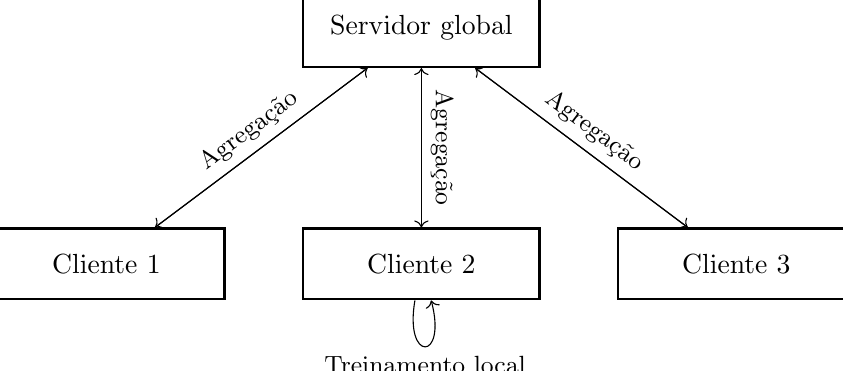
\begin{tikzpicture}[
    server/.style={rectangle, draw, thick, minimum width=3cm, minimum height=1cm, align=center},
    client/.style={rectangle, draw, thick, minimum width=3cm, minimum height=0.9cm, align=center},
    arrow/.style={->, thin}
]

\path[use as bounding box] (-5,-3) rectangle (5,1);

\node[server] (server) at (0,1)
{Servidor global};

\node[client] (c1) at (-4,-2) {Cliente 1};
\node[client] (c2) at (0,-2)  {Cliente 2};
\node[client] (c3) at (4,-2)  {Cliente 3};

\draw[arrow] (server) edge node[midway, above, sloped]{\small Agregação}  (c1);
\draw[arrow] (server) edge node[midway, above, sloped]{\small Agregação} (c2);
\draw[arrow] (server) edge node[midway, above, sloped]{\small Agregação}  (c3);

\draw[arrow] (c1) -- (server);
\draw[arrow] (c2) -- (server);
\draw[arrow] (c3) -- (server);

\draw[->, looseness=6, out=175, in=190]
(c1) edge node[left]{\small Treinamento local} (c1);

\draw[->, looseness=10, out=-100, in=-75]
(c2) edge node[below]{\small Treinamento local} (c2);

\draw[->, looseness=6, out=5, in=-10]
(c3) edge node[right]{\small Treinamento local} (c3);

\end{tikzpicture}
\caption{Fluxo básico do aprendizado federado.}\label{fig:federated_learning}
\end{figure}
\newpage\textbf{Diferenciação.} 
\begin{enumerate}
\item\textbf{Com relação à partição dos dados.} 
A classificação mais tradicional do federated learning diz respeito à forma como os dados estão distribuídos entre as entidades participantes. 
Conforme sistematizado por Zhang et al.~\cite{zhang2021survey}, 
essa categorização pode ser dividida em três cenários principais:
\begin{enumerate}
\item\textit{Aprendizado federado horizontal.}  
Nesse cenário, os conjuntos de dados possuem funcionalidades semelhantes, porém usuários distintos, 
isto é, há grande sobreposição no espaço de atributos, mas pouca interseção no espaço de instâncias. 
A partição ocorre ao longo das linhas da base de dados. 
Esse modelo é amplamente utilizado em aplicações como teclados inteligentes e sistemas de recomendação distribuídos, 
sendo o FedAvg~\cite{mcmahan2017communication} o algoritmo de agregação mais comum~\cite{zhang2021survey}.

\item\textit{Aprendizado federado vertical.}  
Aqui ocorre o oposto: os usuários são majoritariamente os mesmos, enquanto as funcionalidades são distintas. 
A partição é feita ao longo das colunas do conjunto de dados. 
Esse cenário é comum em colaborações interinstitucionais, como entre bancos e empresas de e-commerce, 
onde diferentes entidades possuem informações complementares sobre os mesmos usuários. 
Nesse contexto, técnicas baseadas em criptografia homomórfica e alinhamento seguro de entidades são amplamente utilizadas\cite{hardy2017private,cheng2021secureboost}.

\item\textit{Aprendizado federado com transferência.}  
Quando há pouca sobreposição tanto de usuários quanto de funcionalidades, 
recorre-se a técnicas de aprendizado por transferência para viabilizar o treinamento colaborativo. 
Esse modelo é particularmente útil em cenários com dados escassos ou rotulados de forma incompleta, 
como aplicações de classificação de imagem ou modelos de aprendizado de linguagem natural~\cite{yang2020}.
\end{enumerate}

\item\textbf{Com relação aos mecanismos de privacidade.} 
Embora o federated learning evite o compartilhamento direto dos dados brutos, 
a troca de parâmetros de modelo ainda pode levar ao vazamento de informações sensíveis. 
Dessa forma, diferentes mecanismos de privacidade são empregados:
\begin{enumerate}
\item\textit{Agregação segura de modelos.}  
Baseia-se na combinação de parâmetros locais sem que o servidor tenha acesso às atualizações individuais. 
Protocolos de \textit{secure aggregation} garantem que apenas o modelo global agregado seja observável~\cite{bonawitz2017practical}.

\item\textit{Criptografia homomórfica.}  
Permite que operações matemáticas sejam realizadas diretamente sobre dados criptografados, 
garantindo que nem o servidor nem outros participantes tenham acesso às informações originais. 
Esse método é comum em aprendizado federado vertical~\cite{hardy2017private,zhang2021survey}.

\item\textit{Privacidade diferencial.}
Consiste na adição controlada de ruído estatístico aos gradientes ou parâmetros do modelo, 
limitando a possibilidade de inferência sobre dados individuais. 
Pode ser aplicada tanto local quanto globalmente e é amplamente utilizada em sistemas reais, 
como os propostos e estudados pelo Google~\cite{mcmahan2018learning,bonawitz2019towards}.
\end{enumerate}

\item\textbf{Com relação ao modelo de aprendizado de máquina aplicado.} 
O federated learning não se restringe a um tipo específico de modelo, 
sendo aplicável a diferentes classes de algoritmos de aprendizado de máquina:
\begin{enumerate}
\item\textit{Modelos lineares.}  
Incluem regressão linear, regressão logística e ridge regression. 
Modelos lineares, como regressão linear e ridge regression, 
são frequentemente utilizados como ponto de partida em ambientes federados devido à sua simplicidade algorítmica e eficiência computacional, 
especialmente em cenários com restrições de privacidade e comunicação~\cite{nikolaenko2013privacy,zhang2021survey}.

\item\textit{Modelos baseados em árvores.}  
Árvores de decisão, random forests e gradient boosting têm sido adaptados para o contexto federado, 
especialmente em ambientes verticais. 
O SecureBoost é um exemplo representativo desse tipo de abordagem~\cite{cheng2021secureboost}.

\item\textit{Redes neurais profundas.}  
Redes neurais são amplamente utilizadas em aplicações modernas de federated learning, 
como reconhecimento de voz, visão computacional e sistemas embarcados. 
Frameworks baseados em FedAvg permitem o treinamento eficiente de redes profundas em larga escala~\cite{mcmahan2017communication,bonawitz2019towards}.
\end{enumerate}

\item\textbf{Com relação aos métodos de tratamento da heterogeneidade.} 
A heterogeneidade dos dados e dos recursos de clientes é um dos principais desafios inerente aos ambientes distribuídos,
que pode manifestar-se tanto na forma de dados estatisticamente 
não-IID\footnote{dados não-IID violam uma ou ambas dessas seguintes propriedades: independência e distribuição idêntica.
Assim, dados não-IID podem ser um sinal de que ou há viés no conjunto de dados, ou de que os dados não seguem a mesma distribuição,
ou de que há correlação local entre os dados. 
Uma vez que cada cliente coleta dados de acordo com comportamentos e contextos específicos,
resultando em distribuições distintas entre dispositivos, dados não-IID são um comum em aprendizado federado.}
quanto em diferenças computacionais,
de disponibilidade e de conectividade entre os dispositivos participantes.
Diversos mecanismos têm sido propostos na literatura para mitigar esses efeitos adversos:
\begin{enumerate}
\item\textit{Comunicação assíncrona.}
Abordagens assíncronas permitem que o servidor agregue atualizações de clientes à medida que elas se tornam disponíveis,
sem a necessidade de sincronização global entre todos os participantes.
Esse modelo reduz o impacto de \textit{stragglers} e dispositivos com conectividade intermitente,
sendo particularmente adequado para cenários em larga escala e ambientes móveis~\cite{zhang2021survey}.

\item\textit{Amostragem de clientes.}
Em sistemas federados reais, apenas um subconjunto dos clientes disponíveis participa de cada rodada de treinamento.
A amostragem de clientes reduz significativamente os custos de comunicação e computação,
além de tornar o processo mais robusto à heterogeneidade de recursos.
Esse mecanismo é parte fundamental do algoritmo FedAvg e de seus desdobramentos~\cite{mcmahan2017communication}.

\item\textit{Mecanismos tolerantes a falhas.}  
Falhas de comunicação, desconexões inesperadas e clientes lentos são comuns em ambientes federados.
Métodos tolerantes a falhas buscam garantir a continuidade do treinamento e preservar propriedades de convergência
mesmo na presença de clientes ausentes ou atualizações perdidas.
Embora fora do escopo do aprendizado federado supervisionado tradicional,
trabalhos em Federated Reinforcement Learning (FRL), como o de Fan et al.~\cite{fan2022fault},
formalizam esse problema e propõem estratégias que mantêm a estabilidade do treinamento
sob diferentes modelos de falha.

\item\textit{Heterogeneidade de modelos e aprendizado personalizado.}  
Para lidar com distribuições de dados altamente não-IID, abordagens de aprendizado federado personalizado
permitem a coexistência de modelos locais adaptados a cada cliente juntamente com um modelo global compartilhado.
O trabalho de Liang et al.~\cite{liang2020think} propõe a separação entre representações globais e locais,
reduzindo o impacto da heterogeneidade estatística e melhorando o desempenho individual dos clientes.
\end{enumerate}
\end{enumerate}

\section{Geração de Dados Sintéticos}\label{sec:synthetic}
A escassez de dados de alta qualidade, combinada com regulamentações rigorosas de privacidade e o alto custo de anotação manual, impulsionou a adoção da geração de dados sintéticos como uma alternativa viável aos \textit{datasets} reais~\cite{lu2023}. 
Dados sintéticos são definidos como informações artificialmente geradas por algoritmos ou simulações que mimetizam as propriedades estatísticas e comportamentais dos dados reais, sem conter informações diretamente identificáveis. No contexto de sistemas de Inteligência Artificial seguros e privados, a geração de dados sintéticos não atua apenas como uma ferramenta de aumento de dados (\textit{data augmentation}), mas como um mecanismo fundamental de preservação de privacidade e robustez\cite{goyal2024}.
\subsection{Técnicas de Geração Baseadas em IA Generativa}
A literatura recente categoriza as abordagens de geração de dados sintéticos principalmente em três arquiteturas de aprendizado profundo:
\begin{enumerate}
    \item \textbf{Redes Adversárias Generativas (GANs):} Consistem em dois modelos neurais, um gerador e um discriminador, que competem entre si. O gerador cria dados falsos e o discriminador tenta distinguir entre dados reais e falsos. GANs são amplamente utilizadas para síntese de imagens e dados tabulares, com variantes aplicadas especificamente para preservar a estrutura estatística de dados sensíveis~\cite{goyal2024}.
    \item \textbf{Autoencoders Variacionais (VAEs):} Os VAEs aprendem a comprimir os dados de entrada em um espaço latente probabilístico e, em seguida, reconstróem os dados a partir desse espaço, permitindo a amostragem de novos pontos de dados que seguem a distribuição original~\cite{lu2023}.
    \item \textbf{Grandes Modelos de Linguagem (LLMs):} Avanços recentes, como apontado por Nadăş et al.~\cite{nadas2025}, demonstram que LLMs podem atuar como geradores de dados universais para texto e código. 
    Através de técnicas de \textit{prompting} e refinamento iterativo, LLMs podem gerar dados rotulados e código sintético verificável via execução, 
    auxiliando no treinamento de modelos de segurança de software.
\end{enumerate}
\subsection{Sinergia com Mecanismos de Privacidade e Segurança}
A geração de dados sintéticos desempenha um papel estratégico quando integrada às técnicas de \textit{Differential Privacy}, \textit{Federated Learning} e \textit{Machine Unlearning}.

\subsubsection{Privacidade Diferencial (DP).}
A aplicação direta de modelos gerativos em dados sensíveis pode resultar em riscos de privacidade, como ataques de inferência de pertinência (\textit{membership inference attacks}). Para mitigar isso, a geração de dados sintéticos é frequentemente acoplada à Privacidade Diferencial~\cite{lu2023}. 
O objetivo é gerar um \textit{dataset} sintético que preserve as propriedades estatísticas globais, mas garanta que a saída do modelo não dependa excessivamente de nenhum registro individual. Técnicas como DP-GAN integram ruído calibrado garantindo garantias formais de privacidade ($\epsilon$-differential privacy), permitindo que dados sintéticos sejam compartilhados publicamente com risco minimizado.

\subsubsection{Aprendizado Federado (FL).}
No Aprendizado Federado, a heterogeneidade dos dados é um desafio crítico. A geração de dados sintéticos oferece soluções em duas frentes~\cite{goyal2024}:
\begin{enumerate}
    \item \textbf{Aumento de Dados Local:} Clientes com poucos dados podem usar modelos generativos para sintetizar amostras locais, melhorando a robustez do treinamento.
    \item \textbf{Privacidade Generativa Federada:} O treinamento de GANs em ambiente federado, onde apenas os parâmetros dos geradores são compartilhados, permite que o modelo global aprenda a distribuição de dados sem acesso direto aos registros brutos.
\end{enumerate}

\subsubsection{Machine Unlearning.}
O \textit{Machine Unlearning} visa remover a influência de dados específicos de um modelo treinado. A geração de dados sintéticos atua como facilitador neste processo:
\begin{enumerate}
    \item \textbf{Prevenção de Memorização:} O uso de dados sintéticos treinados com DP desde o início reduz a necessidade de \textit{unlearning} frequente, pois os dados não correspondem a indivíduos reais.
    \item \textbf{Substituição de Dados:} Em cenários onde dados reais devem ser excluídos, dados sintéticos podem ser gerados para preencher a lacuna estatística deixada pela remoção, mantendo a utilidade do modelo sem violar a privacidade~\cite{nadas2025}.
\end{enumerate}
\section{Conclusão}

A crescente dependência de sistemas de Inteligência Artificial em diversos setores da sociedade trouxe à tona questões fundamentais sobre a proteção de dados pessoais e a conformidade com regulamentações de privacidade.
Neste trabalho, apresentamos uma revisão sistemática das principais técnicas de preservação de privacidade aplicadas ao contexto de aprendizado de máquina, explorando suas características, aplicações e limitações.

Conforme discutido ao longo deste \textit{survey}, o \textit{federated learning} emerge como
uma solução robusta para cenários onde a centralização de dados é inviável
ou indesejável. Ao manter os dados nos dispositivos locais e compartilhar apenas parâmetros de modelo, essa abordagem reduz significativamente os riscos de vazamento
de informações sensíveis. No entanto, como demonstrado, a simples descentralização não é suficiente. A heterogeneidade de dados não-IID, as limitações de comunicação e os
potenciais ataques de inferência sobre gradientes compartilhados exigem
mecanismos adicionais de proteção.

Nesse contexto, a privacidade diferencial atua como uma camada complementar
de segurança, fornecendo garantias formais e quantificáveis sobre o nível
de privacidade preservado. A adição controlada de ruído estatístico aos dados ou aos parâmetros do  modelo limita a capacidade de adversários inferirem informações sobre
indivíduos específicos, mesmo quando têm acesso ao modelo treinado.
Essa técnica, quando integrada ao aprendizado federado, fortalece
substancialmente as garantias de privacidade do sistema como um todo.

O \textit{machine unlearning}, por sua vez, responde a uma demanda regulatória e
ética cada vez mais presente: o direito ao esquecimento.
A capacidade de remover seletivamente a influência de dados específicos
de modelos já treinados, sem comprometer significativamente seu desempenho,
representa um avanço importante na direção de sistemas de IA mais
transparentes e responsáveis. Embora ainda existam desafios técnicos consideráveis, especialmente em
relação à eficiência computacional e às garantias de remoção completa,
os métodos discutidos neste trabalho demonstram a viabilidade prática
dessa abordagem.

A geração de dados sintéticos, como explorado na Seção~\ref{sec:synthetic}, desempenha um
papel estratégico ao complementar as técnicas anteriores.
Ao produzir dados artificiais que preservam propriedades estatísticas
relevantes sem expor informações individuais, essa abordagem não apenas
facilita o compartilhamento de dados para pesquisa e desenvolvimento,
mas também oferece soluções para problemas de escassez de dados e
desbalanceamento de classes.
A sinergia entre geração de dados sintéticos e privacidade diferencial,
em particular, permite a criação de datasets públicos com garantias
formais de privacidade.

\textbf{Desafios e direções futuras.}
Apesar dos avanços significativos nas técnicas de preservação de privacidade,
diversos desafios permanecem em aberto.
A tensão fundamental entre utilidade do modelo e nível de privacidade
garantido continua sendo um ponto crítico de pesquisa.
Em muitos cenários práticos, a adição de ruído ou a descentralização do
treinamento resulta em degradação de desempenho que pode ser inaceitável
para aplicações críticas.

Além disso, a composição de múltiplas técnicas de privacidade, embora
promissora, introduz complexidades adicionais em termos de análise de
garantias e overhead computacional.
A integração de federated learning com privacidade diferencial e machine
unlearning, por exemplo, requer cuidadosa calibração de parâmetros e
análise de trade-offs.

Outro desafio importante diz respeito à escalabilidade dessas técnicas
para cenários de larga escala.
Embora frameworks como o proposto por Bonawitz et al.~\cite{bonawitz2019towards}
demonstrem a viabilidade do aprendizado federado com milhões de dispositivos,
questões relacionadas a custos de comunicação, tolerância a falhas e
heterogeneidade de recursos permanecem como obstáculos práticos.

Por fim, a avaliação rigorosa de garantias de privacidade em sistemas
reais continua sendo um problema em aberto.
Ataques cada vez mais sofisticados, como os de inferência de pertinência
e reconstrução de dados, demonstram que garantias teóricas nem sempre se
traduzem em proteção efetiva contra adversários determinados.

\textbf{Considerações finais.}
As técnicas de preservação de privacidade discutidas neste \textit{survey}
representam avanços fundamentais na direção de sistemas de IA mais
seguros e responsáveis.
A combinação de \textit{federated learning}, \textit{differential privacy}, \textit{machine unlearning}
e geração de dados sintéticos oferece um conjunto robusto de ferramentas
para diferentes cenários e requisitos de privacidade.
No entanto, a adoção prática dessas técnicas ainda enfrenta barreiras
técnicas, regulatórias e organizacionais que demandam esforços contínuos
de pesquisa e desenvolvimento.
À medida que regulamentações de privacidade se tornam mais rigorosas e
a conscientização sobre proteção de dados aumenta, espera-se que essas
técnicas se tornem componentes essenciais de qualquer sistema de IA
implantado em ambientes de produção.

% teste
% ---- Bibliography ----
%
% BibTeX users should specify bibliography style 'splncs04'.
% References will then be sorted and formatted in the correct style.ss
%
\bibliographystyle{splncs04}
\bibliography{refs}

%
\end{document}
